\begin{history}

    \enquote{Immer vorwärts}, so heisst die Parole unserer Musikgesellschaft.
    Stillstand heisst Rückgang. 1955 besuchte man das Kantonale Musikfest in
    Malters und 1957 das Eidgenössische in Zürich. Ebenso vertrat der Verein an
    den Musiktagen von Hitzkirch und Littau, sowie am Schwyzer
    Kantonal-Musikfest in Brunnen unsere Gemeinde. Dass Musik keine politischen
    Grenzen kennt, zeigt uns die Einladung nach Aidlingen (Stuttgart) zum
    dortigen Bezirksmusikfest

    Eine besondere Anerkennung möchten wir unseren Dirigenten widmen. Ihr
    Bestreben ist, den musikalischen Stand des Vereins zu heben und die
    Leistungen zu verbessern. Mit grossen Fähigkeiten und eisernem Willen gelang
    es ihnen, die Musikgesellschaft Hildisrieden musikalisch weiter
    emporzuführen. In ihren Bestrebungen fanden sie stets ungeteilte und
    geschlossene Unterstützung durch Vorstand und Musikanten. Wenn es trotzdem
    hin und wieder kleine Trübungen gab, so waren sie sicher nicht allzu ernst
    gemeint, denn das Wohl und die Ehre des Vereins standen immer im
    Vordergrund, Ihre Ratschläge, ihre grosse Aufopferung und Treue zur
    Musikgesellschaft verdient aufrichtigen Dank.

    Der schönste Brauch im Vereinsleben ist die Pflege des geselligen und
    kameradschaftlichen Lebens durch gegenseitigen Besuch. Da werden die
    freundschaftlichen Bande unter den Musikvereinen enger geknüpft. Die Besuche
    der Stadtmusik Laufen im Jahre 1952, der Harmonie Neuenkirch 1961, sowie
    jener der Aidlinger Blaskapelle 1972 freuten uns sehr. So werden alte, liebe
    Freundschaftsbande aufgefrischt und neue angebahnt. Möge dieser schöne
    Brauch immer erhalten bleiben.

    Die seit 1953 alljährlich im Hildisriederwald stattfindenden Waldfeste
    stärken die Vereinskasse (denn dieser Anlass wird nicht des Festes wegen
    organisiert). Dieser Anlass verursacht den Musikanten viel Mühe und Arbeit,
    ist aber bei der Bevölkerung sehr beliebt, wie der gute Besuch immer
    beweist. Die heissen Sommertage locken die Musikfreunde in den kühlen Wald,
    um bei Musik und Tanz einige gemütliche Stunden zu geniessen.

    Der 3. Juli 1954 war ein ganz besonderer Tag für die Musikgesellschaft,
    Unter dem Motto \enquote{Zoge am Boge} konzertierten wir in einer
    volkstümlichen Sendung im Radiostudio Basel, nebst dem Jodelklub Pilatus,
    Luzern, und dem Handharmonika-Duett Lustenberger, Emmenbrücke. Der schöne
    Erfolg gab dem Verein den nötigen Impuls für die Weiterreise nach Laufen zur
    dortigen Stadtmusik, um an der Jubiläumsfeier teilzunehmen. Die
    Feierlichkeiten eröffneten die Musikgesellschaft Konkordia Allschwil, der
    Männerchor Laufen und schliesslich die Hildisrieder Musikanten. Die
    musikalischen Darbietungen, sowie die humoristischen Einlagen von Mathias
    Jutz als Conferencier ernteten rauschenden Beifall. Im September gleichen
    Jahres durften wir die Grenzbesetzungssoldaten der Mitr Kp. 4 mit einem
    Konzert erfreuen

    Trotz Schneegestöber am Auffahrtsmorgen vom 19. Mai 1955, wurde dann der
    Abend zu einer sehr eindrucksvollen Feier. Der Empfang zu Ehren des neu
    gewählten Regierungsrates Dr. Werner Bühlmann war ein einmaliges Erlebnis

    Die Musikgesellschaft ist 1955 auf 31 Mitglieder angewachsen, und der
    Vorstand setzte sich wie folgt zusammen:

    Präsident: Hans Troxler, Ausserbuchen Aktuar: Kaspar Troxler, Moos Kassier:
    Josef Rüttimann, Dorf Mat.-Verwalter: Otto Estermann, Traselingen Beisitzer:
    Hans Suppiger, Dorf

    1956 wirkte unser Verein an der Luzerner-Fasnacht mit. Die Musikanten waren
    als Zahnärzte verkleidet. Der zahlenmässig erstarkte Verein stand 1957 vor
    der Wahl einer neuen Uniform. Mit tatkräftiger Unterstützung seitens der
    vielen Gönner konnte die Neuuniformierung beschlossen werden.

    Mit dem neuen Kleid zogen unsere Musikanten erstmals an das eidgenössische
    Musikfest in Zürich. Neben vielen Proben und Auftritten gehört hin und
    wieder eine verdiente, gemütliche Reise ins Programm, um die Kameradschaft
    zu beleben. Wir erinnern an die Ausflüge an den Rheinfall 1950, ins
    Bündnerland 1952, ins Tessin 1956, auf die Rigi 1958, ins Urnerland 1960,
    ins Lötschental 1962, auf die Schwägalp 1964, in das Engadin 1967, die
    Drei-See-Rundfahrt 1969 und die Reise auf die Riederund Bettmeralp 1972.

    Da viele Musikanten zu den besten Schützen unserer Gemeinde zählen, ist es
    für die Musikgesellschaft stets eine Freude, diese bei der Heimkehr von
    grossen Schützenfesten feierlich zu empfangen. Am Freundschaftstreffen 1961
    mit der Harmonie Neuenkirch in Neuenkirch übergab Präsident Silvester
    Troxler seinen Musikfreunden die Ehrenurkunde.

    Am 24. Februar 1962 konzertierten unsere Musikanten zur Eröffnung des
    neuerbauten Gasthof zum Roten Löwen und ebenso im November zum Antrinket im
    renovierten Restaurant Kreuz.

    Der 29. November 1962 war ein denkwürdiger Tag für unser Dorf, Regierungsrat
    Franz Xaver Leu übergab die neue Dorfstrasse dem Verkehr. Dem Dorfausbau
    mussten neun Häuser weichen. Der \enquote{Vierwaldstätterhof}, als`grösstes
    Verkehrshindernis, war lange Zeit ein dankbares Fasnacht-Sujet, das
    allerdings schon Jahre vorher vom unvergesslichen Mathis Jutz mehrmals
    entrümpelt wurde.

    Die Generalversammlung vom 12. März 1966 beschloss die Neuanschaffung von
    Instrumenten. Man kaufte 7 Flügelhörner à Fr. 580.—, 2 Euphonium zu Franken
    1350.—, 1 Es-Bass à Fr. 2200,— der Marke Wilson von Kurath, Flums, sowie 5
    Courtois-Trompeten A Fr. 530.—.

    Im Sommer 1970 erlebten die Hildisrieder einen Pfarrauftritt, Dekan Josef
    Jost von Beromünster, vorher Pfarrer in Hochdorf wurde Pfarrherr von
    Hildisrieden. An der Delegiertenversammlung des Kantonalen Musikverbandes
    1972 in Kriens wurde der Musiktag Hildisrieden übertragen.

    Kann man sich ein Fest denken ohne Musik? Nach meiner Auffassung sicher
    nicht. Wo immer die Klänge einer Musik ertönen, herrscht froher Sinn und
    Gemütlichkeit. Wohin auch die Musikgesellschaft Hildisrieden gerufen wird,
    ist sie bereit, mitzumachen. Mit besonderer Freude folgt sie jeweils den
    Einladungen von Nachbarsektionen zu einer Banneroder Uniformweihe.

    Die Stadtmusik Laufen, mit der sie freundschaftliche Beziehungen pflegt,
    rief sie zu einem Gala-Konzert. Ein Kurplatzkonzert in Luzern zu geben und
    mit ihren Darbietungen Gäste aus aller Welt zu erfreuen, zählt zu ihren
    dankbaren Ereignissen. Die Hildisrieder-Fasnacht beleben und der
    Götschizunft eine Freude zu bereiten beweist, dass sie auch Verständnis für
    echtes Brauchtum hat. Auch andere Feste verschönern, gehört zu ihrer
    Aufgabe. Mit den Vereinen von Hildisrieden begeht sie nach vollendetem
    Tagewerk den 1. August.

    So oft der hochwürdige Bischof zur Firmung unsere Gemeinde besuchte, oder
    ein Pfarrer oder Primiziant Einzug hielt, fehlte auch das zu ihren Ehren
    gegebene Ständchen auf dem Dorfplatz nicht.

    Ein schöner Brauch, den der Verein pflegt, ist, den neuvermählten Kameraden
    ein Ständchen zu bringen. Die gleiche Aufmerksamkeit wird auch den verehrten
    Jubilaren anlässlich des Geburtstages oder der Goldenen Hochzeit zuteil. Oft
    schon stand die Musikgesellschaft am Grabe eines lieben Aktiv oder
    Ehrenmitgliedes. Wehmutsvoll senkte sich jeweils das Vereinsbanner unter den
    Klängen des letzten Musikgrusses in die kühle Gruft. Auch die grösseren und
    kleineren Ausmärsche in die nähere Umgebung, die speziell unseren Gönnern
    und Freunden gewidmet sind, und die sich zur Ausbildung in der Marschmusik
    eignen, seien hier erwähnt. Wir schön, dass die Musikgesellschaft nach dem
    Motto handelt: \enquote{In Freud und Leid, zum Spiel bereit.}

    \subsubsection*{Dritte Fahnen-und zweite Uniformweihe 1957}

    Es war nicht ganz einfach, für die Musikgesellschaft Hildisrieden eine neue
    Fahne zu entwerfen, denn es ging ja nicht nur um ein mehr oder weniger
    dekoratives Zeichen, das hin und wieder hervorgeholt wird. Die Fahne
    bedeutet ihr mehr. Sie ist nach wie vor das Feldzeichen, um das sich Männer
    scharen. Dem Wunsch aller Musikanten entsprechend, wurde der Entwurf
    Professor Boesch, vom Schloss Heidegg, einem anerkannten Historiker
    anvertraut. Sein Sujet fand begeisterte Aufnahme. Er zeigt das
    Gemeindewappen als Zeichen der Zusammengehörigkeit und ein Musikinstrument
    auf blauem Grund, das Symbol der Musik. Die Farben in weiss, rot und blau
    gehalten, dokumentieren Gemeinde- und Kantonsfarben. Das mächtige Banner
    wurde mit viel Liebe im Kloster Eschenbach angefertigt.

    Der Neu-Uniformierung voraus ging ein von Haus-zu-Haus-Ständchen. Wir waren
    uns im klaren, dass die ganze Angelegenheit der Finanzierung der Mithilfe
    der ganzen Bevölkerung bedarf. Um so mehr freute es uns, dass wir überall
    mit viel Verständnis empfangen wurden. Ein reichhaltiges Angebot an
    Uniformen und Stoffen erschwerte die Auswahl. Sieger blieb schlussendlich
    die Firma Gränicher \& Cie., Luzern, die uns die Kleidung in Stahlbau
    lieferte. Die Begeisterung der Musikanten für die Uniform war verständlich.
    Die Kosten von Fr. 17 875.— oder Fr. 450.— pro Uniform konnten durch eine
    Sammlung aufgebracht werden. Die grosse Sympathie, die die Musikgesellschaft
    geniesst, hat somit ihre Bestätigung erfahren.

\end{history}

\begin{figure}[ht]
    \subfloat[Neuuniformierung und Fahnenweihe 1957]{%
        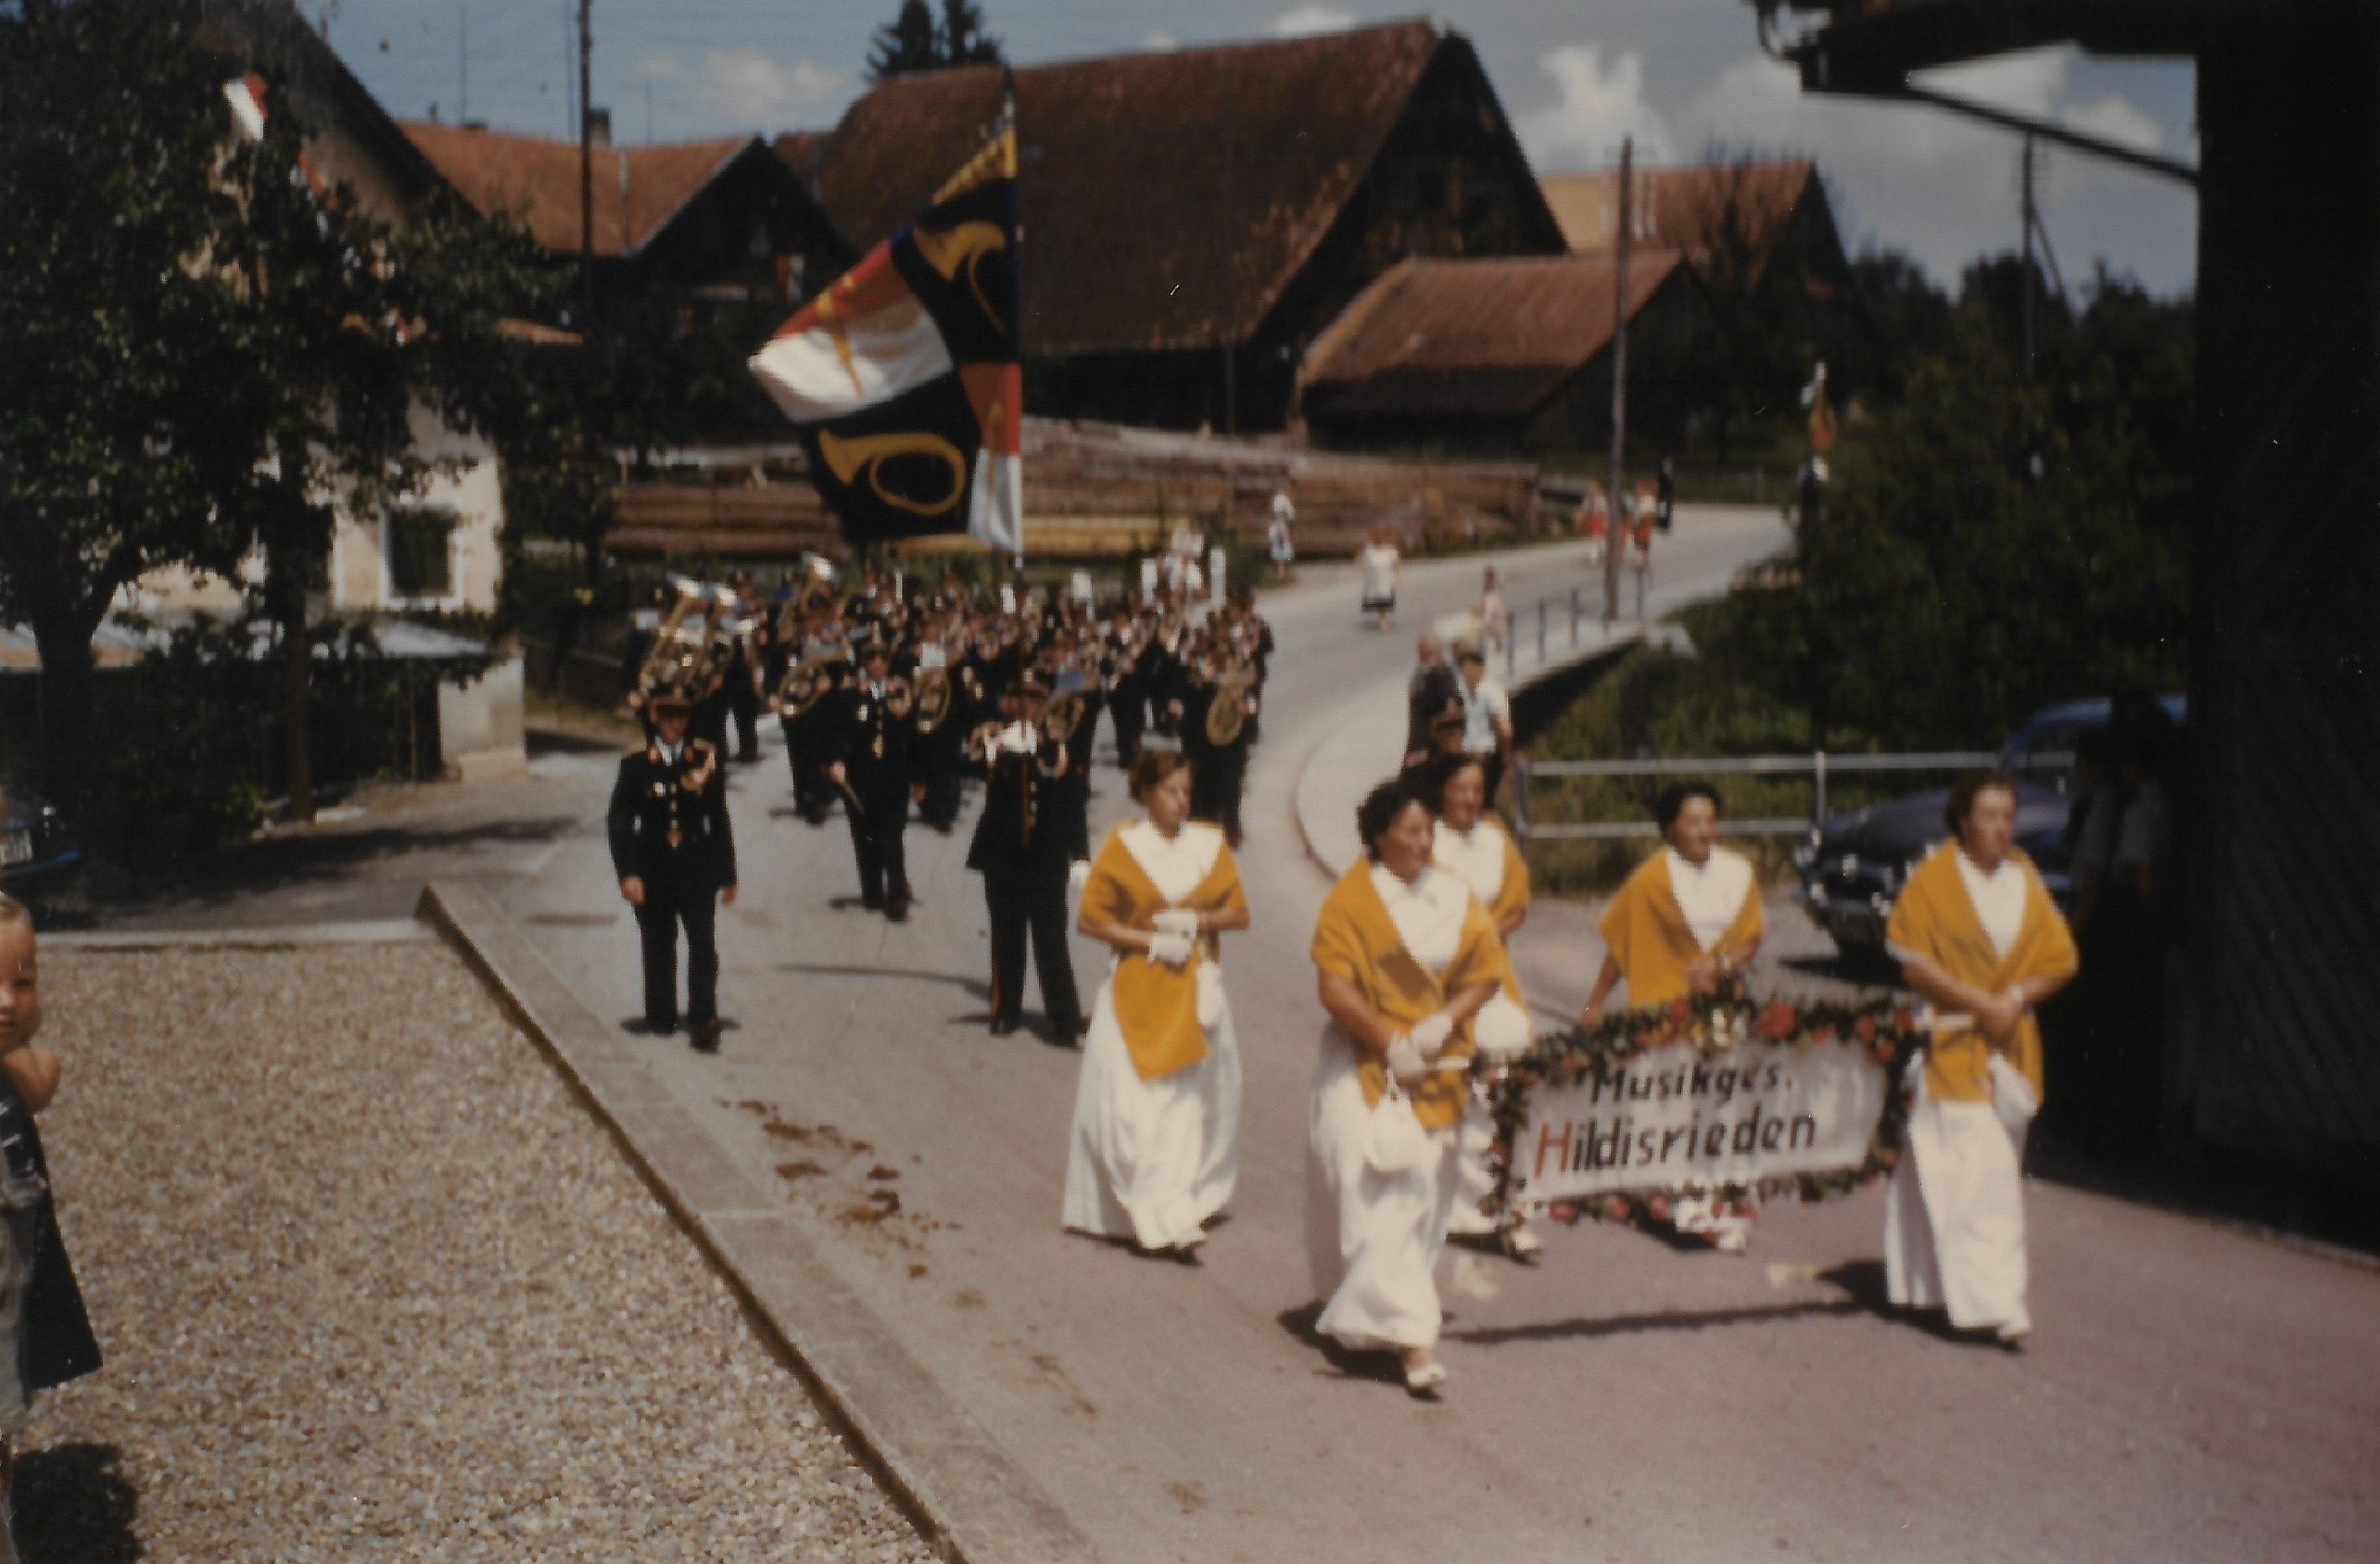
\includegraphics[width=0.48\textwidth,keepaspectratio]{./chap/1950-1974/MGH-Neuuniformierung-1957.jpg}
    }\hfil \subfloat[Um 1965]{%
        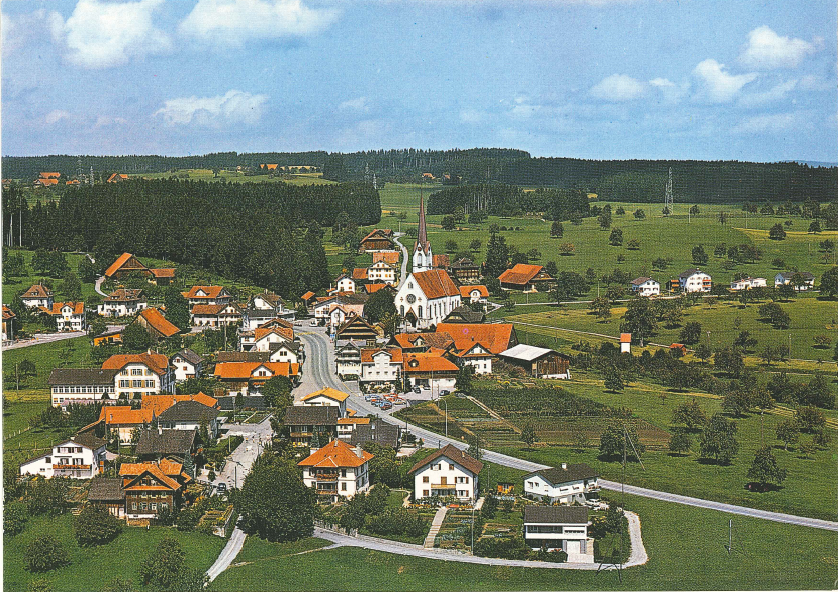
\includegraphics[width=0.45\textwidth,keepaspectratio]{./Dorf-Bilder/p13}
    }\\
    \subfloat[Eidg. Musikfest Zürich 1957]{%
        \includegraphics[width=0.48\textwidth,keepaspectratio]{./chap/1950-1974/1958/MGH-1958-Zürich.jpg}
    }\hfil \subfloat[Luftaufnahme von Hildisrieden 1965]{%
        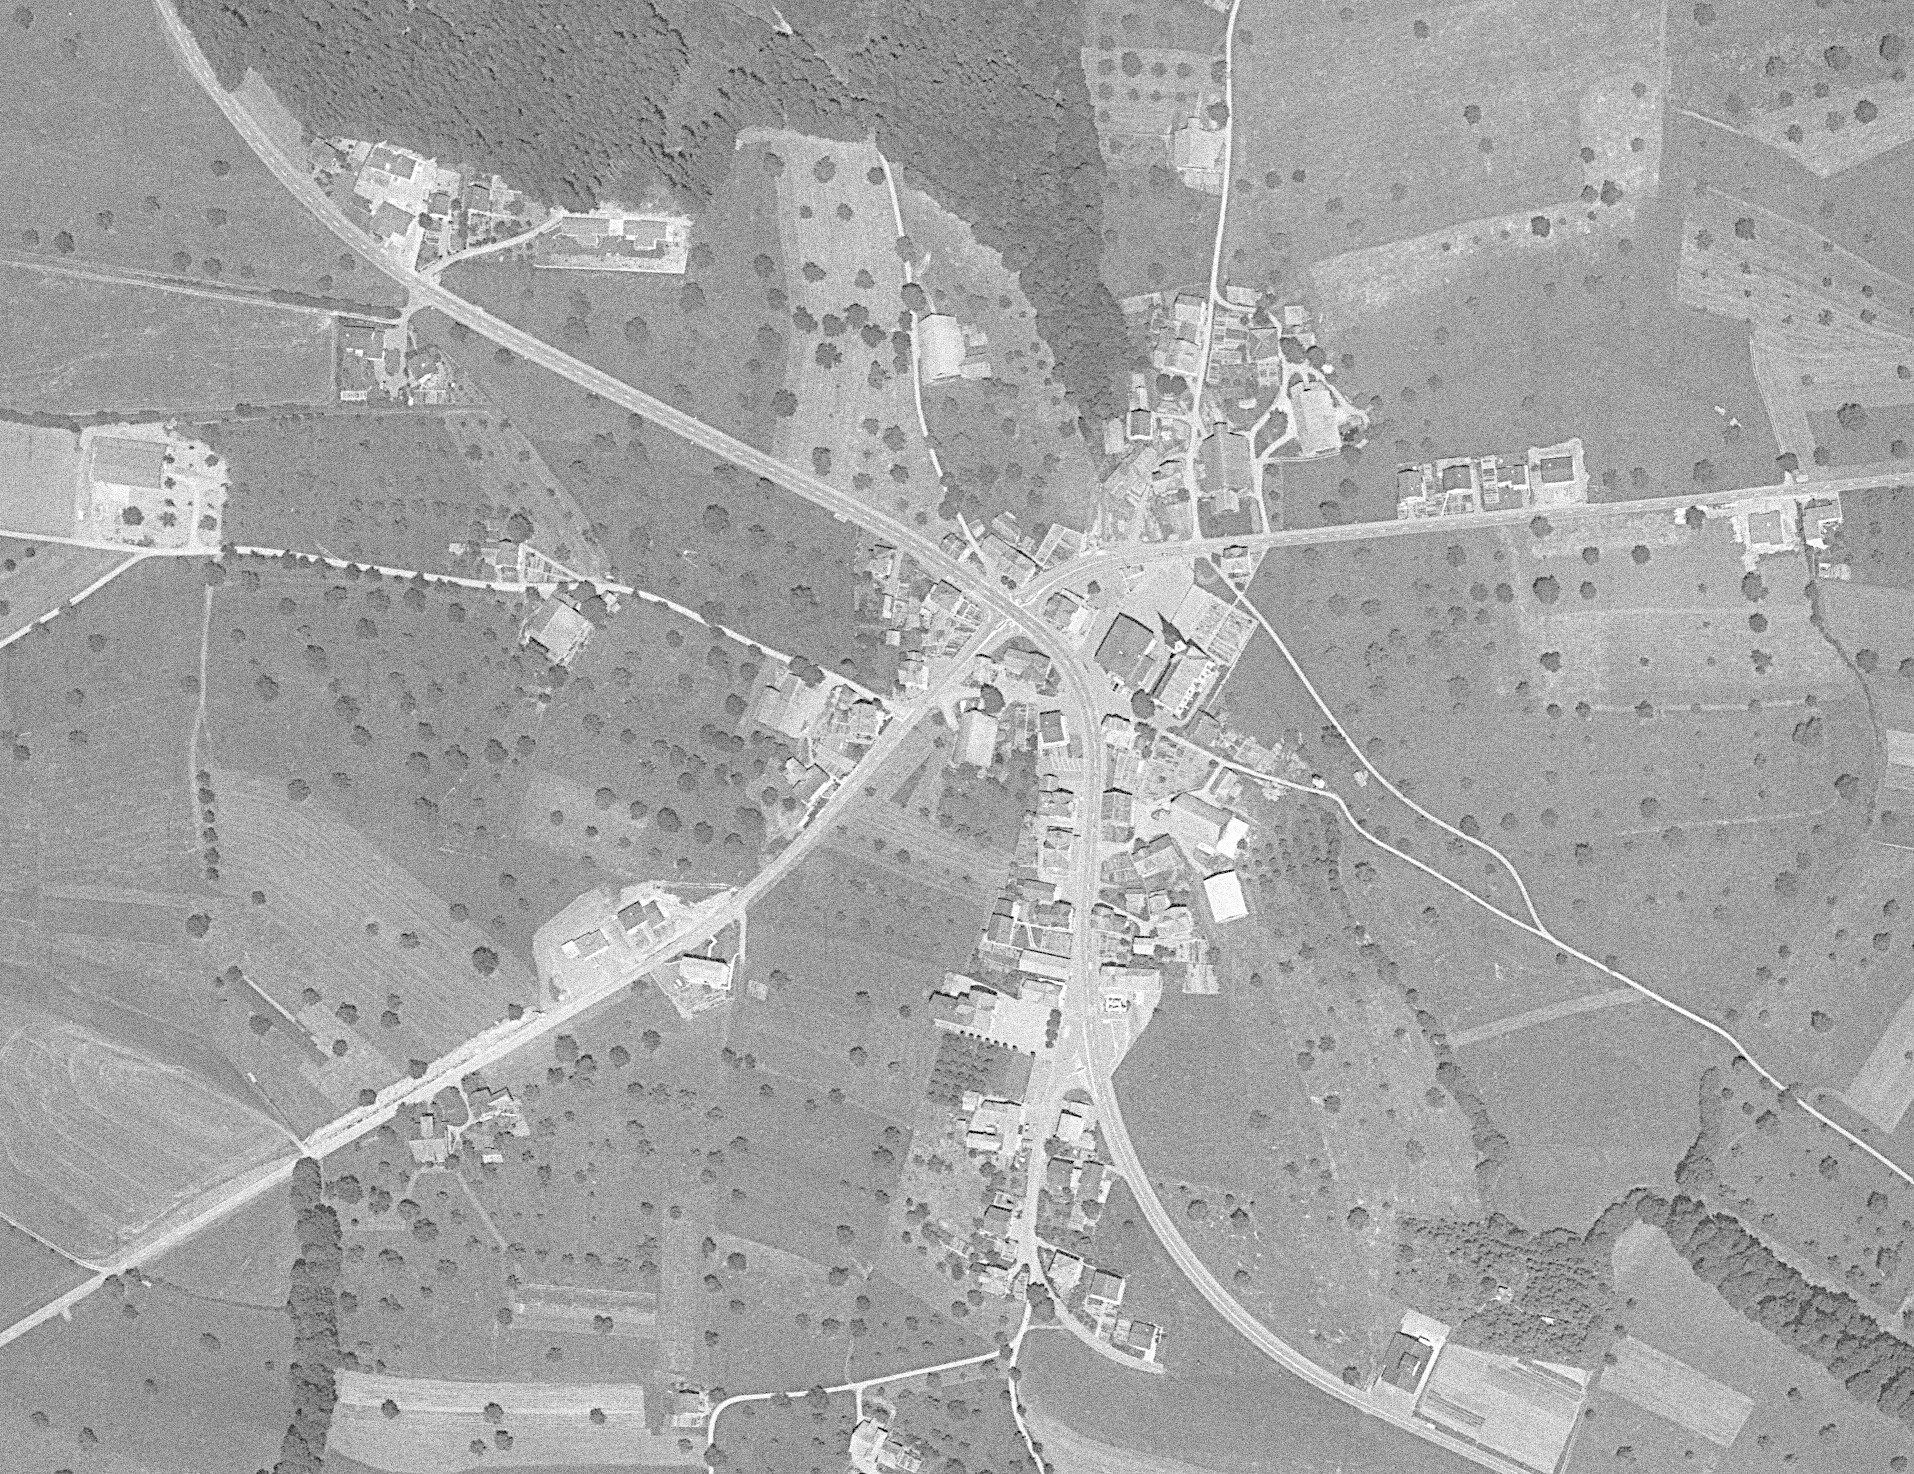
\includegraphics[width=0.45\textwidth,keepaspectratio]{./Dorf-Bilder/Luftaufnahme-1965.jpg}
    }
\end{figure}

\groupphoto{1.0}{1.0}{./chap/1950-1974/1958/MGH-1958.jpg}
{\emph{Die Muskikgesellschaft 1958}\\
    Sitzend:\\
    Troxler Jakob, Suppiger Hans, Estermann Leo, Distel Anton, Amrein Josef,
    Suter Fridolin, Bründler Josef, Troxler Kaspar, Estermann Otto, Estermann
    Leo\\
    1. Reihe:\\
    Gassmann Alois, Troxler Josef, Troxler Franz, Troxler Hermann, Troxler Hans,
    Sommerhalder Albert, Dirigent, Estermann Alois, Käppeli Hans, Käppeli Jakob,
    Troxler Silvester, Troxler Hans\\
    2. Reihe:\\
    Muri Otto, Estermann Hans, Gassmann Josef, Wolf Franz, Rüttimann Josef,
    Schmid Alois, Estermann Franz, Estermann Anton, Troxler Stefan, Troxler
    Karl, Kramis Alois\\
    3. Reihe:\\
    Suter Jakob, Winiger Hans, Fleischli Josef, Steffen August, Wolf Josef }
{fig:mgh-1958}

\clearpage

\begin{history}

    \subsubsection*{Kant. Musiktag vom 5. und 6. Mai 1973}

    Erstmals in der Geschichte durfte die Musikgesellschaft Hildisrieden einen
    Kant. Musiktag durchführen. Über 1200 Musikanten aus allen Gauen des
    Luzernerbietes haben Hildisrieden die Ehre erwiesen. Am 5. und 6. Mai trafen
    sich 28 stramme Musikkorps zu einem imposanten Musiktreffen. Ohne Kränze und
    Ehrenmeldungen, aber mit einem sachlichen Expertenbericht, gibt der Musiktag
    den Vereinen eine Standortbestimmung.

    Bereits am Samstagnachmittag stellten sich die Musikgesellschaften zu den
    Wettspielvorträgen in der Turnhalle, so die Musikgesellschaft Römerswil,
    Harmonie Rickenbach, Feldmusik Grosswangen, die Harmonien Sempach und
    Beromünster, die Musikgesellschaften Littau und Reiden, um anschliessend zur
    Marschmusik auf der Strasse anzutreten. Am Samstagabend herrschte
    Feststimmung beim grossen Galakonzert der Feldmusik Grosswangen unter der
    Leitung von Hans Känzig.

    Die erstaunlich guten Musikvorträge vor den Experten wurden am
    Sonntagvormittag von den Vereinen Hitzkirch, Eschenbach, Neudorf,
    Rothenburg, Eintracht Schötz, Rickenbach, Buttisholz, Feldmusik Neuenkirch,
    Zell, Perlen-Buchrain, St. Urban, Feldmusik Rain, Ermensee, Grossdietwil,
    Frohsinn Grosswangen, Hergiswil, Gunzwil, Ballwil, Harmonie Rain, Harmonie
    Neuenkirch und Schwarzenbach fortgesetzt. Die vielen Proben haben sich
    gelohnt. Die luzernische Blasmusik steht mit sehr gutem Nachwuchs auf
    solidem Boden. Die zahlreichen Besucher beklatschten die rassige
    Marschmusik-Demonstration vom Sonntagnachmittag.

    Der schneidige OK-Präsident Julius Bieri stellte in seiner
    Begrüssungsansprache fest, dass sich die Luzerner Vereine auf dem Gebiete
    des Blasmusikwesens auf einer beachtlichen Stufe befinden. Auch
    Kantonalpräsident Leo Köpfli zeigte sich im angefüllten Festzelt begeistert:
    \enquote{Ich danke den Organisatoren und der Gemeinde Hildisrieden für die
        gelungene Durchführung des Musiktages, sowie den Interpreten für ihre
        hervorragenden Leistungen.}

    Fast hundert Veteranen konnten von der Festgemeinde durch den Veteranenchef
    Anton Fischer, Reiden, geehrt werden. Hildisrieden hat es verstanden, den
    Kant. Musiktag als musikalisches Testfest zu gestalten und zu einem
    unterhaltsamen Ereignis zu machen. Die grosse Teilnahme am Fest ist ein
    Beweis grossen Vertrauens, was wir sehr zu schätzen wussten.

    \subsubsection*{100-Jahr Feier und dritte Uniformweihe am 4. 5. und 7. Mai 1974}

    Das Jubiläumsfest beginnt mit einem festlichen Eröffnungskonzert am
    Samstagabend, an dem die alte, stahlblaue Uniform mit rassigen Klängen
    verabschiedet wird. Der befreundete Musikverein Aidlingen aus Deutschland
    gibt ein Galakonzert in der zum Bersten gefüllten Festhalle und bringt auch
    das Bierzelt mit Stimmungsmusik auf jubilierende Hochstimmung.

    Mit der Totenehrung auf dem Friedhof beginnt das sonntägliche Programm, und
    der Marsch \enquote{alte Kameraden} erklang in den Sonntagmorgen. Der
    feierliche Gottesdienst gibt dem Fest einen würdigen Anfang.

    Nachher trifft man sich zum gemütlichen Frühschoppenkonzert, vorgetragen von
    Musikverein Aidlingen. Die Vorträge der Stadtmusik Laufen umrahmen das
    Bankett. Der farbenfrohe Einzug der geladenen Musikvereine aus der Umgebung
    sowie die alte und neue Uniform bildeten den Höhepunkt des Festes. Die
    Veteranen wurden durch den Vereinspräsidenten Fritz Disler mit Nelken und
    weissem Wein geehrt aus Dankbarkeit für die vielen Verdienste dies die dem
    Verein hergaben.

    Das Fest dehnt sich am Sonntagabend weiter aus. Als Stargast konzertiert die
    Musikgesellschaft Engelberg, welche zum grossartigen Ambiente im Festzelt
    beiträgt und viel Applaus ernteten.

    Am Schlussabend der Geburtstagsparty zeigt sich das musikalische Können der
    Musikgesellschaft Hildisrieden unter der Leitung von Franz Limacher. Der
    unermüdliche Aschi Lehmann versteht es vorzüglich, die Feststimmung noch
    einmal so richtig zu heben.

\end{history}

\groupphoto{0.93}{0.8}{./chap/1950-1974/1974/MGH-1974.jpg}
{\emph{Neuuniformierung 1974}\\
    1. Reihe:\\
    Stierli Marcel, Achermann Albert, Estermann Alois, Troxler Hermann,
    Estermann Leo, Dörig Franz, Limacher Franz, Direktor, Troxler Kaspar, Dörig
    Kaspar, Bieri Andreas, Estermann Otto, Koller Alois, Troxler Silvester\\
    2. Reihe:\\
    Arnold Franz, Gassmann Josef, Estermann Klaus, Luterbach Erwin, Disler Fritz, Dörig
    Markus, Estermann Franz, Luterbach Walter, Gassmann Alois sen., Portmann
    Anton, Troxler Werner\\
    3. Reihe:\\
    Wolf Franz, Suter Jakob, Troxler Hans, Rüttimann Franz, Estermann Anton,
    Rüttimann Josef, Rüttimann Walter, Estermann Hans, Troxler Walter\\
    4. Reihe:\\
    Troxler Karl, Rüttimann Herbert, Troxler Edgar, Estermann Bruno, Estermann
    Edy, Estermann Franz, Estermann Hugo, Wolf Josef, Gassmann Alois jun., Balmer Beat }
{fig:mgh-1974}